\documentclass[border=4pt]{standalone}
\usepackage{tikz}
\usepackage{amsmath,amssymb}
\usetikzlibrary{arrows.meta,positioning,calc,fit,backgrounds}
\definecolor{ink}{HTML}{0B0B0B}\definecolor{ink2}{HTML}{52514E}\definecolor{muted}{HTML}{898781}
\definecolor{axis}{HTML}{C3C2B7}\definecolor{wash}{HTML}{F0EFEC}\definecolor{blue}{HTML}{2A78D6}
\definecolor{orange}{HTML}{EB6834}\definecolor{red}{HTML}{E34948}\definecolor{aqua}{HTML}{1BAF7A}
\begin{document}
\sffamily\small
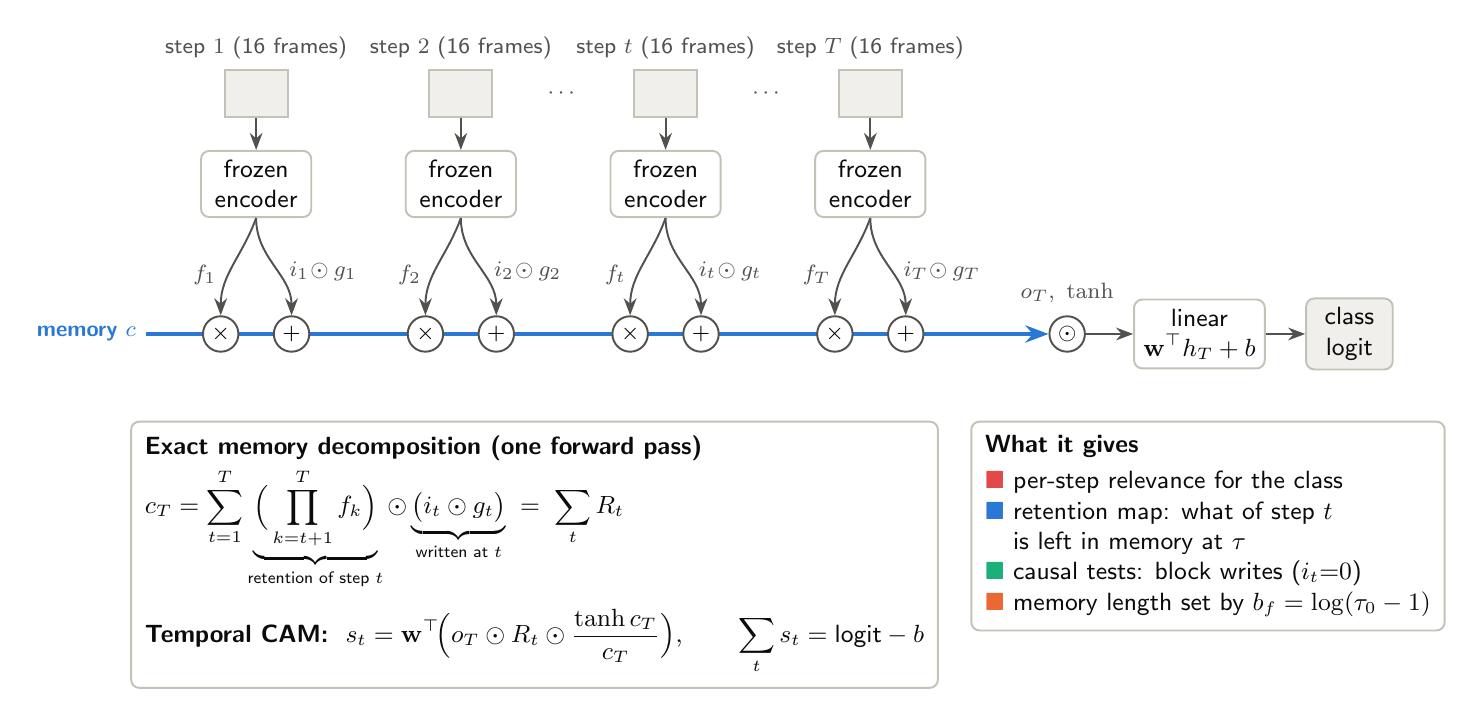
\begin{tikzpicture}[
  >=Stealth, line width=0.7pt, font=\sffamily\small,
  box/.style={draw=axis, rounded corners=3pt, fill=white, minimum height=7mm, align=center, text=ink},
  frame/.style={draw=axis, fill=wash, minimum width=8mm, minimum height=6mm},
  op/.style={circle, draw=ink2, fill=white, inner sep=0.6pt, minimum size=4.5mm, font=\sffamily\footnotesize},
  lbl/.style={text=ink2, font=\sffamily\footnotesize}]
% ------------------------------------------------ top: model
\foreach \i/\t in {1/1,2/2,3/t,4/T}{
  \node[frame] (f\i) at (2.6*\i,4.6) {};
  \node[lbl, above=0pt of f\i] {step $\t$ (16 frames)};
  \node[box, below=4mm of f\i, minimum width=14mm] (e\i) {frozen\\ encoder};
  \draw[->, ink2] (f\i) -- (e\i);
}
\node[lbl] at ($(f3)!0.5!(f4)$) {$\cdots$};
\node[lbl] at ($(f2)!0.5!(f3)$) {$\cdots$};
% memory line
\coordinate (m0) at (1.2,1.55);
\coordinate (mEnd) at (12.0,1.55);
\draw[blue, line width=1.6pt] (m0) -- (mEnd);
\node[text=blue, anchor=east, font=\sffamily\footnotesize\bfseries] at (m0) {memory $c$};
\foreach \i/\t in {1/1,2/2,3/t,4/T}{
  \node[op] (x\i) at ($(e\i.south |- m0)+(-0.45,0)$) {$\times$};
  \node[op] (p\i) at ($(e\i.south |- m0)+(0.45,0)$) {$+$};
  \draw[->, ink2] (e\i.south) to[out=-90,in=90] node[pos=0.55, right, lbl, xshift=1pt] {$i_{\t}\!\odot g_{\t}$} (p\i);
  \draw[->, ink2] (e\i.south) to[out=-110,in=90] node[pos=0.6, left, lbl, xshift=-1pt] {$f_{\t}$} (x\i);
}
% ------------------------------------------------ readout
\node[op] (oT) at (12.9,1.55) {$\odot$};
\node[lbl, above=1pt of oT] {$o_T,\ \tanh$};
\node[box, right=6mm of oT, minimum width=13mm] (fc) {linear\\ $\mathbf{w}^{\top}h_T+b$};
\node[box, right=5mm of fc, minimum width=11mm, fill=wash] (y) {class\\ logit};
\draw[->, blue, line width=1.2pt] (mEnd) -- (oT);
\draw[->, ink2] (oT) -- (fc); \draw[->, ink2] (fc) -- (y);
% ------------------------------------------------ bottom: decomposition
\node[box, align=left, anchor=north west, minimum width=10.2cm, inner sep=5pt] (dec) at (1.0,0.45) {%
  \textbf{Exact memory decomposition (one forward pass)}\\[2pt]
  $c_T=\displaystyle\sum_{t=1}^{T}\underbrace{\Big(\prod_{k=t+1}^{T} f_k\Big)}_{\text{retention of step }t}\odot\underbrace{\big(i_t\odot g_t\big)}_{\text{written at }t}\;=\;\sum_{t} R_t$\\[6pt]
  \textbf{Temporal CAM:}\ \ $s_t=\mathbf{w}^{\top}\!\Big(o_T\odot R_t\odot\dfrac{\tanh c_T}{c_T}\Big),\qquad \displaystyle\sum_t s_t=\text{logit}-b$};
\node[box, align=left, anchor=north west, inner sep=5pt, minimum width=5.6cm] (uses) at ($(dec.north east)+(4mm,0)$) {%
  \textbf{What it gives}\\[2pt]
  \textcolor{red}{$\blacksquare$}\ per-step relevance for the class\\
  \textcolor{blue}{$\blacksquare$}\ retention map: what of step $t$\\ \hphantom{$\blacksquare$}\ is left in memory at $\tau$\\
  \textcolor{aqua}{$\blacksquare$}\ causal tests: block writes ($i_t{=}0$)\\
  \textcolor{orange}{$\blacksquare$}\ memory length set by $b_f=\log(\tau_0-1)$};
\end{tikzpicture}
\end{document}
